% readme.tex -- a short example of how each Stata Journal insert should be
% organized.

\inserttype{article}

\author{Short article author list}{%
  Daoping Wang\\
  School of Urban and Regional Science,\\ 
  Shanghai University of Finance and Economics\\
  Shanghai, China\\
  daopingwang@live.sufe.edu.cn\\
  \\

  \and
  Kerui Du\\
  School of Management, Xiamen University\\
  Xiamen, China\\
  kerrydu@xmu.edu.cn \\
  \\
  
  \and
  Ning Zhang\\
  Institute of Blue and Green Development, Shandong University\\
  Weihai, China\\
  zn928@naver.com
}

\title[Short toc article title]{Measuring technical efficiency and total factor productivity change with undesirable outputs in Stata}
\maketitle


\begin{abstract}
	In this article, we introduce two user-written data envelopment analysis commands for measuring technical efficiency and productivity change in Stata. Over the last decades, an important theoretical progress of data envelopment analysis, a nonparametric method widely used for performance assessment of decision-making units, is the incorporating of undesirable outputs. Models with the ability to deal with undesirable outputs have been developed and applied in empirical studies for assessing the sustainability of decision-making units, and are getting more and more attention from researchers and managers. The {\tt teddf} command developed in the present article allows users to measure technical efficiency, both radial and non-radial, when some outputs are undesirable. Technical efficiency measures are obtained by solving linear programming problems. The {\tt gtfpch} command provides tools for measuring productivity change, e.g., the Malmquist-Luenberger index and the Luenberger indicator. We provide a brief overview of the nonparametric efficiency and productivity change measurement with the consideration of undesirable outputs, and we describe the syntax and options of the new commands. Examples are given to illustrate how to perform the technical efficiency and productivity analysis with the newly introduced commands.
	
	\keywords{teddf, gtfpch, DEA, Malmquist-Luenberger index, Luenberger indicator, directional distance function, total fatcor productivity}
\end{abstract}


% discussion of the Stata Journal document class.
%\input sj.tex
% discussion of the Stata Press LaTeX package for Stata output.
%\input stata.tex

\section{Introduction}\label{sec_intro}
%[background]
After the pioneering work of \cite{Farrell1957}, \cite{Debreu1951}, and \cite{koopmans1951analysis}, efficiency and productivity analysis have been widely used in empirical studies assessing the performance of decision-making units (DMUs) in terms of converting inputs into outputs. 
Among the parametric and nonparametric frontier models that have been developed in the field of efficiency analysis, Data Envelopment Analysis (DEA) has received plenty of attention for its no needing for prior information of the production function form and capability in multiple output technologies \citep{Fare1985,Fare1994}. 
Efficiency analysis based on DEA is usually assumed that inputs should be shrunk and outputs should be expanded. However, in the real
world, outputs are not always desirable. In the case of undesirable outputs, they should be shrunk to improve efficiency.
In the last decades, with the increasing demand for improving the sustainability of the economic society, scholars and managers gradually recognized that it is vital to consider undesirable output in efficiency and productivity analysis \citep{Chung1997,Mahlberg2011}. Correspondingly, DEA models with the ability to deal with undesirable outputs have been developed and applied in empirical studies, e.g., \citep{Zhou2012,Lin2015}. 

%[introduce existing estimation procedures]
The estimation of nonparametric frontier models can be readily performed in Stata with some user-written commands. 
The {\tt dea} command proposed in \cite{Ji2010} provided a basic tool to estimate radial technical efficiency using the DEA technique in Stata. 
\cite{Badunenko2016} extended {\tt dea} with five new commands that allow users to implement both radial and nonradial technical efficiency estimation, as well as statistical inference in nonparametric frontier models in Stata. 
\cite{Tauchmann2012} introduced two commands, i.e., {\tt orderm} and {\tt orderalpha}, for implementing order-$m$, order-$\alpha$, and free disposal hull efficiency analysis in Stata. 
%[gap]
These commands mentioned above, however, are limited in their capability for performing efficiency and productivity analysis with undesirable outputs. 

%[introduce the command provided here]
Here, we introduce two user-written commands for measuring technical efficiency and productivity change with undesirable outputs in Stata. {\tt teddf} estimates directional distance function (DDF) with undesirable outputs for technical efficiency measurement. Both radial Debreu-Farrell and nonradial Russell measures can be calculated under different assumptions about the production technology, e.g., window, biennial, sequential, and global production technology.
{\tt gtfpch} measures total factor productivity (TFP) change with undesirable outputs using the Malmquist–Luenberger productivity index or the Luenberger indicator. 
%[advantages]
The new commands open up the possibility to do efficiency and productivity analysis with undesirable outputs in Stata in an effortless way, and their results can directly feed to other Stata routines for further analysis. 

%[structure of the present paper]
The remainder of this article unfolds as follows: 
section \ref{sec_method} provides a brief overview of the nonparametric efficiency and productivity change measurement with the consideration of undesirable outputs; 
sections \ref{sec_teddf} and \ref{sec_gtfpch} contain the syntax and explain the options of {\tt teddf} and {\tt gtfpch}, respectively; 
section \ref{sec_example} presents a hypothetical example to show the usage of the two commands; 
and section \ref{sec_conclusion} concludes the article.

\section{The model}\label{sec_method}
%[intro]
In this section, we provide a brief overview of the nonparametric efficiency and productivity measurement with the consideration of undesirable outputs. 
The radial and nonradial directional distance function will be introduced firstly, followed by the description of the measurement of technical efficiency and TFP change using DDFs. 
The exposition here is only introductory. For more details, please refer to the cited works.

\subsection{Directional distance function}
Consider a production unit transforming a vector of nonnegative inputs into a vector of nonnegative desirable outputs and a vector of by-products (undesirable outputs) such as pollution, subject to the constraint imposed by a fixed technology. For the production technology, inputs and desirable outputs are supposed to be strongly disposable. The undesirable outputs are assumed to be weakly disposable, which indicates that the decrease of undesirable outputs is not free but will lead to a deduction in desirable outputs.
If we denote the input, desirable output, and undesirable outputs as $\pmb{x} \in \Re _ + ^N$,  $\pmb{y} \in \Re _ + ^M$, and $\pmb{b} \in \Re _ + ^H$, respectively, the production technology described above can be characterized by the technology set as
\begin{equation}\label{eq_tech}
    T = \{ (\pmb{x},\pmb{y},\pmb{b}) : \pmb{x} \text{ can produce } (\pmb{y},\pmb{b}) \}.
\end{equation}

Then, following \cite{Chung1997}, the radial DDF is defined as
\begin{equation}\label{eq_ddf_r}
    D_r (\pmb{x},\pmb{y},\pmb{b};\pmb{g}) = \sup \{ \beta :((\pmb{x},\pmb{y},\pmb{b}) + \beta \pmb{g}) \in T  \} 
\end{equation}
where $\pmb{g} = (\pmb{g}_x,\pmb{g}_y, \pmb{g}_b) \in \Re _ - ^N \times \Re _ + ^M \times \Re _ - ^H$ is a preassigned nonzero vector, specifying the direction in which the distance between the data point, $(\pmb{x},\pmb{y},\pmb{b})$, and the production frontier is measured. 

Equation \eqref{eq_ddf_r} gives out the most general form of radial DDF. One can define the distance between the DMU and the production frontier in a specific direction by setting different $\pmb{g}$. By way of illustration, we consider the cases of  ${\pmb{g}_1} = (\pmb{0},\pmb{y},\pmb{0})$, ${\pmb{g}_2} = (\pmb{0},\pmb{0},-\pmb{b})$, ${\pmb{g}_3} = (\pmb{0},\pmb{y},-\pmb{b})$, which is widely used in literature. 
Figure \ref{fig_ddf} presents hypothetical one-desirable output (e.g., \textit{GDP}) one-undesirable output (e.g., \textit{CO$_2$}) production processes. 
Conceptually, in Fig. \ref{fig_ddf}, $\overline{\textit{AB}}$ and $\overline{\textit{AC}}$ represent the distance when the direction is ${\pmb{g}_1} = (\pmb{0},\pmb{y},\pmb{0})$ and ${\pmb{g}_2} = (\pmb{0},\pmb{0}, - \pmb{b})$, respectively. The former focuses on economic prosperity, while the latter focuses on environmental protection. Similarly, $\overline{\textit{AD}}$ is the distance when the direction is ${\pmb{g}_3} = (\pmb{0},\pmb{y}, - \pmb{b})$, which describes the maximum increase of desirable output while simultaneously reducing the undesirable output along the direction $(\pmb{y}, - \pmb{b})$. 
Intuitively, the smaller the distance, the closer the DMU is next to the production frontier, and the distance is 0 for the DMU which operates on the production frontier.

\begin{figure}[ht]
    \centering
    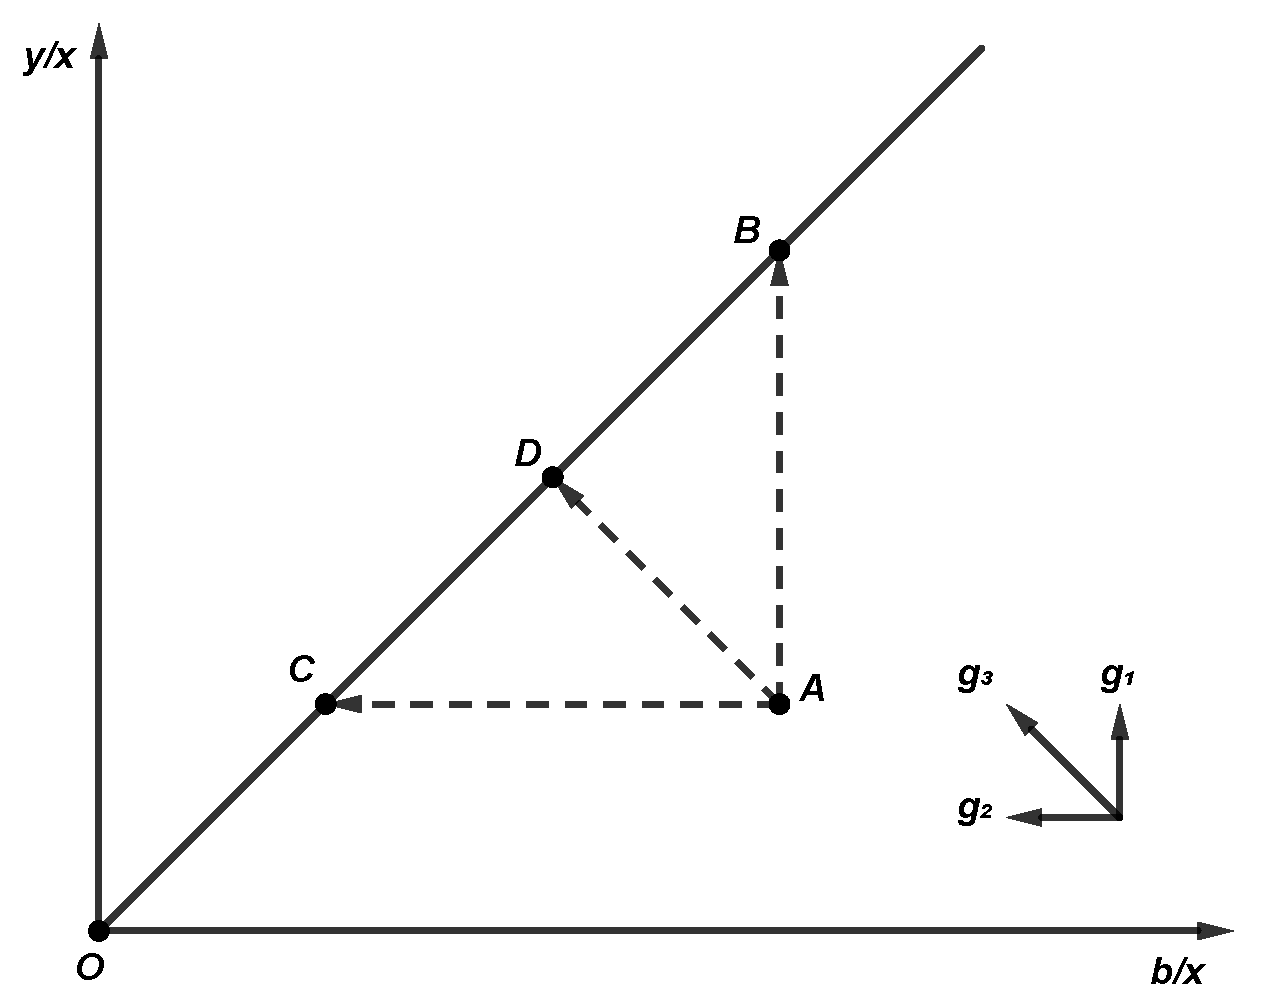
\includegraphics[scale=0.5]{SJF1.pdf}
    \caption{A graphical illustration of directional distance functions} 
    \label{fig_ddf}
\end{figure}

The radial measure expands (shrinks) all outputs or/and inputs proportionally until the production frontier is reached. At the reached frontier point, some but not all outputs (inputs) can be expanded (shrunk) while remaining feasible. If such a possibility is available for a given decision-making unit for some outputs (inputs), then the reference point is said to have slacks in outputs (inputs). Nonradial measures, i.e., the Russell measure, accommodate such slacks \citep{Chambers2002,Fare2010,Zhou2012}.

The nonradial DDF is defined as
\begin{equation}\label{eq_ddf_nr}
    D_{nr} (\pmb{x},\pmb{y},\pmb{b};\pmb{g}) = \sup \{ \pmb{w'} \pmb{\beta} :((\pmb{x},\pmb{y},\pmb{b}) + \textit{diag}(\pmb{\beta}) \cdot \pmb{g}) \in T \} 
\end{equation}
where $\pmb{w}$ denotes a normalized weight vector that is relevant to the numbers of inputs and outputs, and ${\pmb{\beta }} = ({{\pmb{\beta }}_x},{{\pmb{\beta }}_y},{{\pmb{\beta }}_b}) \in {\Re ^N} \times {\Re ^M} \times {\Re ^H}$ denotes the vector of the scaling factors. 
Clearly, the nonradial DDF measure allows the inputs and outputs to be adjusted non-proportionally. Compared with the radial measure in Fig.\ref{fig_ddf}, instead of using a fixed point, e.g., B, C, or D, as the reference point, if the nonradial directional distance function is used, the reference point would be located at any point on the production frontier.
 

\subsection{Measurement of technical efficiency}
To estimate the DDF measure of technical efficiency using the nonparametric technique, the production technology set is derived from observed data. Typically, for the cross-sectional data with $J$ individuals, the production technology set with the assumption of constant return to scale (CRS) is constructed as

\begin{equation}\label{eq_tech_dea}
    T = \left\{ {({\pmb{x}},{\pmb{y}},{\pmb{b}}):\sum\limits_{j = 1}^J {{\lambda _j}{{\pmb{x}}_j} \le {\pmb{x}},\sum\limits_{j = 1}^J {{\lambda _j}{{\pmb{y}}_j} \ge {\pmb{y}},} \sum\limits_{j = 1}^J {{\lambda _j}{{\pmb{b}}_j} = {\pmb{b}},} }  {\pmb{\lambda }} \ge 0} \right\}.
\end{equation}

For variable returns to scale (VRS), $\sum_{j=1}^{J} \lambda_j =1$ is added to the above equation. That is,
\begin{equation}\label{eq_tech_dea_v}
    T = \left\{ {({\pmb{x}},{\pmb{y}},{\pmb{b}}):\sum\limits_{j = 1}^J {{\lambda _j}{{\pmb{x}}_j} \le {\pmb{x}},\sum\limits_{j = 1}^J {{\lambda _j}{{\pmb{y}}_j} \ge {\pmb{y}},} \sum\limits_{j = 1}^J {{\lambda _j}{{\pmb{b}}_j} = {\pmb{b}},} }  {\pmb{\lambda }} \ge 0}, \sum\limits_{j = 1}^J {{\lambda _j} = 1} \right\}.
\end{equation}

In the panel data context, the time-series dimension can provide more information on the production technology. Researchers have proposed different types of production technology sets such as global, sequential, window, biennial, and contemporaneous production technology. The production technology set at the time $t$ as follows:

\begin{equation}\label{eq_tech_dea_panel}
	T(t) = \left\{ {({\pmb{x}},{\pmb{y}},{\pmb{b}}):\sum\limits_{\tau \in \Gamma_t }\sum\limits_{j = 1}^J {{\lambda _{j\tau}}{{\pmb{x}}_{j\tau}} \le {\pmb{x}},\sum\limits_{\tau \in \Gamma_t }\sum\limits_{j = 1}^J {{\lambda _{j\tau}}{{\pmb{y}}_{j\tau}} \ge {\pmb{y}},} \sum\limits_{\tau \in \Gamma_t }\sum\limits_{j = 1}^J {{\lambda _{j\tau}}{{\pmb{b}}_{j\tau}} = {\pmb{b}},} } {\pmb{\lambda }} \ge 0} \right\}.
\end{equation}


The time range, $\tau \in \Gamma_t$, for different types of production technology set are shown in Fig.\ref{fig_time}. In the global production technology, $\tau \in \Gamma_t$ is expressed as $\tau \leq t_{max}$, where $t_{max}$ is the last period in the sample. In the sequential production technology, $\tau \in \Gamma_t$ is expressed as $\tau \leq t$. In the window production technology, $\tau \in \Gamma_t$ is expressed as $t - h \leq \tau \leq t + h $, where $h$ is the bandwidth.  In the biennial production technology, $\tau \in \Gamma_t$ is expressed as $t \leq \tau \leq t + 1 $. In the contemporaneous production technology, $\tau \in \Gamma_t$ is expressed as $\tau=t$. 

\begin{figure}[ht]
    \centering
    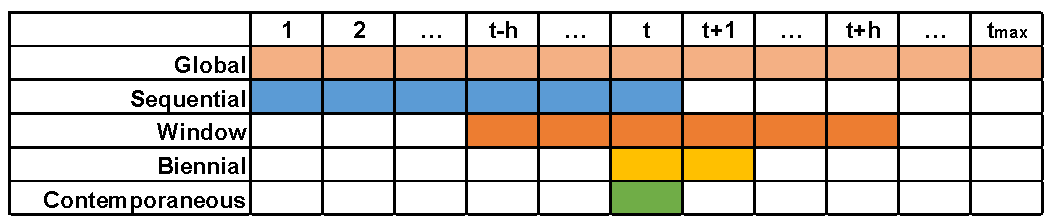
\includegraphics[scale=0.65]{SJF2.pdf}
    \caption{Timing assumption of different type of production technology sets} 
    \label{fig_time}
\end{figure}


Then, the radial DDF measure of inefficiency under the CRS assumption can be estimated by solving the following linear programming problem,
\begin{equation}\begin{split}\label{eq_eff_r}
    D_r (\pmb{x},\pmb{y},\pmb{b};\pmb{g}) 
    = &\max _{\beta,\pmb{\lambda}} \beta  \\ 
    \text{s.t.} &\sum\limits_{j = 1}^J {\lambda _j \pmb{x}_j \le \pmb{x} + \beta \pmb{g}_x}, \\ 
                &\sum\limits_{j = 1}^J {\lambda _j \pmb{y}_j \ge \pmb{y} + \beta \pmb{g}_y}, \\ 
                &\sum\limits_{j = 1}^J {\lambda _j \pmb{b}_j = \pmb{b} + \beta \pmb{g}_b}, \\ 
                &\lambda _j \ge 0, j = 1,...,J.
\end{split}\end{equation}
This technology set is based on the assumption of constant return to scale. For VRS assumption, $\sum_{j=1}^{J} \lambda_j =1$ is added to above constraints.

In Eq.(7), the left-hand side of the constraints construct the production frontier using the convex hull of the observation data and the right-hand side allows the assessed DMU to adjust the inputs ($x$), the desirable outputs ($y$) and undesirable outputs ($b$) alongside the direction of $(g_x,g_y,g_b)$. The directional distance function seeks to maximize the reduction of inputs and undesirable outputs and the expansion of the desirable output in means of $(x+\beta g_x, y+ \beta g_y, b+\beta g_b)$ given the production technology. 

Similarly, the nonradial DDF measure of inefficiency considering the undesirable outputs can be obtained by solving the following linear programming problem.
\begin{equation}\begin{split}\label{eq_eff_nr}
    D_{nr} (\pmb{x},\pmb{y},\pmb{b};\pmb{g}) 
    = &\max _{\pmb{\beta},\pmb{\lambda}} \pmb{w'} \pmb{\beta}  \\ 
    \text{s.t.} &\sum\limits_{j = 1}^J {\lambda _j \pmb{x}_j \le \pmb{x} + diag(\pmb{\beta}_x)\cdot \pmb{g}_x}, \\ 
                &\sum\limits_{j = 1}^J {\lambda _j \pmb{y}_j \ge \pmb{y} + diag(\pmb{\beta}_y)\cdot \pmb{g}_y}, \\ 
                &\sum\limits_{j = 1}^J {\lambda _j \pmb{b}_j = \pmb{b} + diag(\pmb{\beta}_b)\cdot \pmb{g}_b}, \\ 
                &\pmb{\beta} \ge 0; \lambda _j \ge 0, j = 1,...,J.
\end{split}\end{equation}
For variable returns to scale assumption, $\sum_{j=1}^{J} \lambda_j =1$ is added to above constraints. 

Unlike the directional distance function shown in Eq.(7), the nonradial directional distance function allows each component of inputs, desirable outputs, and undesirable outputs to adjust in varying proportions. The nonradial DDF is the maximum weighted sum of the adjustment components ($\beta$) such that $(diag(\beta_x)\cdot g_x,diag(\beta_y)\cdot g_y,diag(\beta_b)\cdot g_b)$ can be produced given the production technology. 


For the panel data case, the radial DDF measure of inefficiency under the CRS assumption can be estimated by solving the following linear programming problem,
\begin{equation}\begin{split}\label{eq_eff_r_panel}
    D_r (\pmb{x},\pmb{y},\pmb{b};\pmb{g}) 
    = &\max _{\beta,\pmb{\lambda}} \beta  \\ 
    \text{s.t.} &\sum\limits_{\tau \in \Gamma_t }\sum\limits_{j = 1}^J {{\lambda _{j\tau}}{{\pmb{x}}_{j\tau}} \le \pmb{x} + \beta \pmb{g}_x}, \\ 
                &\sum\limits_{\tau \in \Gamma_t }\sum\limits_{j = 1}^J {{\lambda _{j\tau}}{{\pmb{y}}_{j\tau}} \ge \pmb{y} + \beta \pmb{g}_y}, \\ 
                &\sum\limits_{\tau \in \Gamma_t }\sum\limits_{j = 1}^J {{\lambda _{j\tau}}{{\pmb{b}}_{j\tau}} = \pmb{b} + \beta \pmb{g}_b}, \\ 
                &\lambda _{j\tau} \ge 0, j = 1,...,J.
\end{split}\end{equation}

Similarly, for the panel data case, the nonradial DDF measure of inefficiency can be estimated by solving the following linear programming problem,
\begin{equation}\begin{split}\label{eq_eff_nr_panel}
    D_{nr} (\pmb{x},\pmb{y},\pmb{b};\pmb{g}) 
    = &\max _{\pmb{\beta},\pmb{\lambda}} \pmb{w'} \pmb{\beta}  \\ 
    \text{s.t.} &\sum\limits_{\tau \in \Gamma_t }\sum\limits_{j = 1}^J {{\lambda _{j\tau}}{{\pmb{x}}_{j\tau}} \le \pmb{x} + diag(\pmb{\beta}_x)\cdot \pmb{g}_x}, \\ 
                &\sum\limits_{\tau \in \Gamma_t }\sum\limits_{j = 1}^J {{\lambda _{j\tau}}{{\pmb{y}}_{j\tau}} \ge \pmb{y} + diag(\pmb{\beta}_y)\cdot \pmb{g}_y}, \\ 
                &\sum\limits_{\tau \in \Gamma_t }\sum\limits_{j = 1}^J {{\lambda _{j\tau}}{{\pmb{b}}_{j\tau}} = \pmb{b} + diag(\pmb{\beta}_b)\cdot \pmb{g}_b}, \\ 
                &\pmb{\beta} \ge 0; \lambda_{j\tau} \ge 0, j = 1,...,J.
\end{split}\end{equation}


\subsection{Measurement of total factor productivity change}
The measurement of productivity change has traditionally focused on measuring marketable (desirable) outputs of DMUs relative to paid factors of production. 
This approach, which typically ignores the production of by-products such as pollution, can yield biased measures of productivity growth \citep{Chung1997}. 
For example, firms in industries that face environmental regulations would typically find that their productivity is adversely affected since the costs of abatement capital would typically be included on the input side, but no account would be made of the reduction in pollutants on the output side.

\cite{Chung1997} has introduced a productivity index based on the radial DDF measure, called the Malmquist-Luenberger productivity index, which credits the reduction of undesirable outputs, e.g., pollution, while simultaneously crediting increases in desirable outputs. Considering two adjacent periods, denoted as $s$ and $t$. respectively. If we choose the direction to be ${\pmb{g}} = (\pmb{0},\pmb{y}, - \pmb{b})$, the output-oriented Malmquist-Luenberger productivity index with undesirable outputs is defined as
\begin{equation}\label{eq_mpi}
    \textit{ML} %_{\pmb{g}} ({{\pmb{x}}^s},{{\pmb{y}}^s},{{\pmb{b}}^s},{{\pmb{x}}^t},{{\pmb{y}}^t},{{\pmb{b}}^t}) 
    = {\left[ {
    \frac{{1 + D _r^t({{\pmb{x}}^s},{{\pmb{y}}^s},{{\pmb{b}}^s};{\pmb{g}})}}{{1 + D _r^t({{\pmb{x}}^t},{{\pmb{y}}^t},{{\pmb{b}}^t};{\pmb{g}})}} \times \frac{{1 + D _r^s({{\pmb{x}}^s},{{\pmb{y}}^s},{{\pmb{b}}^s};{\pmb{g}})}}{{1 + D _r^s({{\pmb{x}}^t},{{\pmb{y}}^t},{{\pmb{b}}^t};{\pmb{g}})}}  } \right]^{1/2}}.
\end{equation}
To avoid an arbitrary choice between base years, an geometric mean of a fraction-based Malmquist-Luenberger productivity index in base year $t$ (first fraction) and $s$ (second fraction) has been taken. The Malmquist–Luenberger measure indicates productivity improvements if their values are greater than one and decreases in productivity if the values are less than one. 

The Malmquist-Luenberger productivity index can be decomposed into two components \citep{Chung1997}, one accounting for efficiency change (\textit{MLEFFCH}), and one measuring technology change (\textit{MLTECH}):
\begin{equation}
    \textit{MLEFFCH} %_{\pmb{g}} ({{\pmb{x}}^s},{{\pmb{y}}^s},{{\pmb{b}}^s},{{\pmb{x}}^t},{{\pmb{y}}^t},{{\pmb{b}}^t}) 
    = \frac{{1 + D _r^s({{\pmb{x}}^s},{{\pmb{y}}^s},{{\pmb{b}}^s};{\pmb{g}})}}{{1 + D _r^t({{\pmb{x}}^t},{{\pmb{y}}^t},{{\pmb{b}}^t};{\pmb{g}})}}
\end{equation}
and,
\begin{equation}
    \textit{MLTECH} %_{\pmb{g}} ({{\pmb{x}}^s},{{\pmb{y}}^s},{{\pmb{b}}^s},{{\pmb{x}}^t},{{\pmb{y}}^t},{{\pmb{b}}^t}) 
    = {\left[ {\frac{{1 + D _r^t({{\pmb{x}}^s},{{\pmb{y}}^s},{{\pmb{b}}^s};{\pmb{g}})}}{{1 + D _r^s({{\pmb{x}}^s},{{\pmb{y}}^s},{{\pmb{b}}^s};{\pmb{g}})}} 
    \times 
    \frac{{1 + D _r^t({{\pmb{x}}^t},{{\pmb{y}}^t},{{\pmb{b}}^t};{\pmb{g}})}}{{1 + D _r^s({{\pmb{x}}^t},{{\pmb{y}}^t},{{\pmb{b}}^t};{\pmb{g}})}}} \right]^{1/2}}.
\end{equation}

Based on the pioneering work in \cite{Chambers2002}, another productivity measure called the Luenberger productivity indicator is also widely used to account for productivity change. 
The Luenberger productivity indicator based on radial DDF measures is defined as
\begin{equation}\begin{split}\label{eq_li_r}
    \textit{L} %({{\pmb{x}}^s},{{\pmb{y}}^s},{{\pmb{b}}^s},{{\pmb{x}}^t},{{\pmb{y}}^t},{{\pmb{b}}^t}) 
    = & \left[ (D _r^t({{\pmb{x}}^s},{{\pmb{y}}^s},{{\pmb{b}}^s};{\pmb{g}}) - D _r^t({{\pmb{x}}^t},{{\pmb{y}}^t},{{\pmb{b}}^t};{\pmb{g}}) \right] \times \frac{1}{2} \\ 
    + & \left[ D _r^s({{\pmb{x}}^s},{{\pmb{y}}^s},{{\pmb{b}}^s};{\pmb{g}}) - D _r^s({{\pmb{x}}^t},{{\pmb{y}}^t},{{\pmb{b}}^t};{\pmb{g}})) \right] \times \frac{1}{2}.
\end{split}\end{equation}
Again, to avoid an arbitrary choice between base years, an arithmetic mean of a difference based Luenberger productivity index in base year $t$ (first difference) and $s$ (second difference) has been taken. 
Productivity improvements are indicated by positive values and declines by negative values. 

In the spirit of decomposition of Malmquist–Luenberger productivity index, the Luenberger productivity indicator based on radial DDFs can also be decomposed into two component measures, i.e., an efficiency change component \citep{Mahlberg2011},
\begin{equation}
    \textit{LEFFCH} %({{\pmb{x}}^s},{{\pmb{y}}^s},{{\pmb{b}}^s},{{\pmb{x}}^t},{{\pmb{y}}^t},{{\pmb{b}}^t}) 
    = D _r^s({{\pmb{x}}^s},{{\pmb{y}}^s},{{\pmb{b}}^s};{\pmb{g}}) - D _r^t({{\pmb{x}}^t},{{\pmb{y}}^t},{{\pmb{b}}^t};{\pmb{g}})
\end{equation}
and a technical change component,
\begin{equation}\begin{split}
    \textit{LTECH} %({{\pmb{x}}^s},{{\pmb{y}}^s},{{\pmb{b}}^s},{{\pmb{x}}^t},{{\pmb{y}}^t},{{\pmb{b}}^t}) 
    = & \left[ D _r^t({{\pmb{x}}^t},{{\pmb{y}}^t},{{\pmb{b}}^t};{\pmb{g}}) - D _r^s({{\pmb{x}}^t},{{\pmb{y}}^t},{{\pmb{b}}^t};{\pmb{g}}) \right] \times \frac{1}{2} \\ 
    + & \left[ (D _r^t({{\pmb{x}}^s},{{\pmb{y}}^s},{{\pmb{b}}^s};{\pmb{g}}) - D _r^s({{\pmb{x}}^s},{{\pmb{y}}^s},{{\pmb{b}}^s};{\pmb{g}}) \right] \times \frac{1}{2}.
\end{split}\end{equation}
The Luenberger indicator based on radial DDFs is expressed as the sum of \textit{LEFFCH} and \textit{LTECH}. \textit{LEFFCH} captures the average gain/loss due to the difference in technical efficiency from period $s$ to period $t$. \textit{LTECH} captures the average gain/loss due to the shift in technology from period $s$ to period $t$.

Like any radial measure of efficiency estimated using DEA technologies, DDF overestimates the efficiency of a firm when there are non-zero slacks that remain in the constraints after the full radial efficiency is achieved. 
To account for these slacks, \cite{Fare2010} proposed a slacks-based measure of efficiency based on nonradial directional distance function. Another type of Luenberger indicator, called the non-proportional Luenberger indicator, can be constructed based on the nonradial DDFs \citep{Mahlberg2011}. 

The Luenberger productivity indicator based on nonradial DDFs is defined as
\begin{equation}\begin{split}\label{eq_li_nr}
    \textit{L} %({{\pmb{x}}^s},{{\pmb{y}}^s},{{\pmb{b}}^s},{{\pmb{x}}^t},{{\pmb{y}}^t},{{\pmb{b}}^t}) 
    = & \left[ (D _{nr}^t({{\pmb{x}}^s},{{\pmb{y}}^s},{{\pmb{b}}^s};{\pmb{g}}) - D _{nr}^t({{\pmb{x}}^t},{{\pmb{y}}^t},{{\pmb{b}}^t};{\pmb{g}}) \right] \times \frac{1}{2} \\ 
    + & \left[ D _{nr}^s({{\pmb{x}}^s},{{\pmb{y}}^s},{{\pmb{b}}^s};{\pmb{g}}) - D _{nr}^s({{\pmb{x}}^t},{{\pmb{y}}^t},{{\pmb{b}}^t};{\pmb{g}})) \right] \times \frac{1}{2}.
\end{split}\end{equation}

The non-proportional Luenberger productivity indicator can also be decomposed into two parts \citep{Mahlberg2011}. An efficiency change component,
\begin{equation}
    \textit{LEFFCH} %({{\pmb{x}}^s},{{\pmb{y}}^s},{{\pmb{b}}^s},{{\pmb{x}}^t},{{\pmb{y}}^t},{{\pmb{b}}^t}) 
    = D _{nr}^s({{\pmb{x}}^s},{{\pmb{y}}^s},{{\pmb{b}}^s};{\pmb{g}}) - D _{nr}^t({{\pmb{x}}^t},{{\pmb{y}}^t},{{\pmb{b}}^t};{\pmb{g}})
\end{equation}
and a technical change component,
\begin{equation}\begin{split}
    \textit{LTECH} %({{\pmb{x}}^s},{{\pmb{y}}^s},{{\pmb{b}}^s},{{\pmb{x}}^t},{{\pmb{y}}^t},{{\pmb{b}}^t}) 
    = & \left[ D _{nr}^t({{\pmb{x}}^t},{{\pmb{y}}^t},{{\pmb{b}}^t};{\pmb{g}}) - D _{nr}^s({{\pmb{x}}^t},{{\pmb{y}}^t},{{\pmb{b}}^t};{\pmb{g}}) \right] \times \frac{1}{2} \\ 
    + & \left[ (D _{nr}^t({{\pmb{x}}^s},{{\pmb{y}}^s},{{\pmb{b}}^s};{\pmb{g}}) - D _{nr}^s({{\pmb{x}}^s},{{\pmb{y}}^s},{{\pmb{b}}^s};{\pmb{g}}) \right] \times \frac{1}{2}.
\end{split}\end{equation}


\subsection{Statistical inference for technical efficiency and productivity index}

Efficiency and productivity analysis are widely applied in benchmarking(relative performance evaluations). The models introduced above are based on the DEA methods which are typically considered to be deterministic. Specifically, the efficiency/productivity is measured relative to the estimated production frontiers constructed by sample observations. Consequently, the measures of efficiency/productivity might be sensitive to the sampling variations. In view of this, researchers have devoted themselves to exploring the statistical properties of the DEA-type estimators. For instance, \cite{banker1993} and \cite{Kneip1998} established consistency and convergence rates of DEA efficiency estimators. \cite{kneip2008} derived the asymptotic distribution of Farrell measure of technical efficiency (one of the radial DEA estimators) in cases with multiple inputs and outputs. Generally speaking, many DEA-type efficiency estimators have been proposed. But few have been known on their asymptotic distribution. 

To implement statistical inference for DEA-type efficiency estimators, \cite{Simar1998} proposed a smoothed bootstrapping procedure. But the consistency of the smooth bootstrapping method has not been proved. Based on the asymptotic theorems developed in \cite{kneip2008}, they presented another two consistent bootstrapping procedures for Farrell measure of technical efficiency: the subsampling approach and the double-smooth bootstrap. \cite{simar2012} showed that the directional distance function estimators shared the known properties of the traditional radial DEA estimators and adapted the subsampling approach and the double-smooth bootstrap to this context. In the context of nonradial DEA estimators, \cite{Badunenko2020} proposed a bootstrap method for Russell measures of technical efficiency. \cite{Badunenko2016} incorporated the bootstrap procedures in their Stata commands {\tt teradialbc} and {\tt tenonradialbc}. It is worth pointing out that the bootstrap methods mentioned above mainly focus on the cross-sectional data. In the panel data cases, there are some difficulties in applying the smooth/double-smooth bootstrapping methods. Because considering the possibility of temporal correlation, they require nonparametric estimation of a high dimensional density which might suffer from the curse of dimensionality. On the contrary, the subsampling approach can be easily adapted to accommodate the panel data structure by subsampling with clusters. Thus, we incorporate the subsampling approach in our Stata command ({\tt teddf}) for statistical inference.

Regarding the statistical inference for DEA-based productivity indexes, \cite{simar2019} established the asymptotic theorems for nonparametric Malmquist indices. \cite{simar1999}  proposed a bootstrap estimation procedure for obtaining confidence intervals for Malmquist indices of productivity and their decompositions. But until now, the statistical properties of the Malmquist-Luenberger productivity index and the Luenberger productivity indicator are still unknown. Intuitively, the subsampling approach can be adapted to these contexts with the knowledge of the convergence rates. Nevertheless, it is still an open issue. 


\endinput

% discussion of the Stata Press LaTeX package for Stata output.

\section{The \textit{teddf} command}\label{sec_teddf}
{\tt teddf} estimates directional distance function with undesirable outputs for technical efficiency measurement.

\subsection{Syntax}
\begin{stsyntax}
	teddf\
	\textit{X\varlist} = \textit{Y\varlist}:\textit{B\varlist} \optif \optin,\
	\underbar{d}mu(\varname)
	\optional{
		    \underbar{t}ime(\varname)
		    gx(\varlist)
		    gy(\varlist)
		    gb(\varlist)
		    \underbar{nonr}adial
		    wmat(name)
		    vrs
		    rf(\varname)
		    \underbar{win}dow(\num)
		    \underbar{bi}ennial 
		    \underbar{seq}uential
		    \underbar{glo}bal
		    brep(\num)
		    alpha(real)
		    tol(real)
		    maxiter(\num)
		    \underbar{sav}ing(filename[,replace])
		    frame(framename)
		    nodots
		    noprint
		    \underbar{noch}eck
 }
\end{stsyntax}


\subsection{Options}

\hangpara
{\tt dmu(\varname)} specifies names of DMUs. It is required.

\hangpara
{\tt time(\varname)} specifies the time variable for panel data.

\hangpara
{\tt gx(\varlist)} specifies direction components for input adjustment. The order of variables specified in gx() should be as the same in \textit{X\varlist}. The \textit{i}th variable in gx() should be the direction of the \textit{i}th variable in \textit{Xvarlist}. By default, gx() takes the opposite of \textit{X\varlist}.

\hangpara
{\tt gy(\varlist)} specifies direction components for desirable output adjustment. The order of variables specified in gy() should be as the same in \textit{Y\varlist}. The \textit{i}th variable in gy() should be the direction of the \textit{i}th variable in \textit{Y\varlist}. By default, gy() takes \textit{Y\varlist}.

\hangpara
{\tt gb(\varlist)} specifies direction components for undesirable output adjustment. The order of variables specified in gb() should be as the same in \textit{B\varlist}. The \textit{i}th variable in gb() should be the direction of the \textit{i}th variable in \textit{B\varlist}. By default, gb() takes the opposite of \textit{B\varlist}.

\hangpara
{\tt nonradial} specifies using the nonradial directional distance measure.

\hangpara
{\tt wmat(name)} specifies a weight matrix for adjustment of input and output variable for the nonradial directional distance measure. The default is wmatrix= (1,...,1).

\hangpara
{\tt vrs} specifies production technology with variable returns to scale. By default, production technology with constant returns to scale is assumed.

\hangpara
{\tt rf(\varname)} specifies the indicator variable that defines which data points of outputs and inputs form the technology reference set.

\hangpara
{\tt window(\num)}  specifies using window production technology with the \num-period bandwidth.

\hangpara
{\tt biennial}  specifies using biennial production technology.

\hangpara
{\tt sequential} specifies using sequential production technology.

\hangpara
{\tt global} specifies using global production technology.

\hangpara
{\tt brep(\num)} specifies the number of bootstrap replications. The default is brep(0) specifying performing the estimator without bootstrap. Typically, it requires 1,000 or more replications for bootstrap DEA methods.

\hangpara
{\tt alpha(real) } sets the size of the subsample bootstrap. By default, alpha(0.7) indicates subsampling $N^{0.7}$ observations out of the $N$ original reference observations.

\hangpara
{\tt tol(real)} specifies the convergence-criterion tolerance  for LinearProgram(). The default value of tol is 1e-8.

\hangpara
{\tt maxiter(\num) } specifies the maximum number of iterations for LinearProgram(). The default value of maxiter is 16000.

\hangpara
 {\tt saving(filename[,replace])}  specifies a filename to store the results.
 
\hangpara
 {\tt frame(name)} specifies a framename to stroe the results.
 
\hangpara
{\tt nodots} suppress iteration dots.

\hangpara
{\tt noprint} suppress suppress display of the results.

\hangpara
{\tt nocheck} suppress checking for new version. It is suggested to be used for saving time when internet connection is unavailable.


\section{The \textit{gtfpch} command}\label{sec_gtfpch}
{\tt gtfpch} measures total factor productivity change with undesirable outputs using Malmquist–Luenberger productivity index or Luenberger indicator.

\subsection{Syntax}
\begin{stsyntax}
	gtfpch\
	\textit{X\varlist} = \textit{Y\varlist}:\textit{B\varlist} \optif \optin,\
	\optional{
		\underbar{d}mu(\varname)
		\underbar{luen}berger
		ort(\ststring)
		gx(\varlist)
		gy(\varlist)
		gb(\varlist)
		\underbar{nonr}adial
		wmat(name)
		\underbar{win}dow(\num)
		\underbar{bi}ennial 
		\underbar{seq}uential
		\underbar{glo}bal	
		fgnz
		rd	
		tol(real)
		maxiter(\num)
		\underbar{sav}ing(filename[,replace])
		frame(framename)
		noprint
		\underbar{noch}eck		
	}
\end{stsyntax}


\subsection{Options}

\hangpara
{\tt dmu(\varname)} specifies names of DMUs. 

\hangpara
{\tt luenberger} specifies estimating Luenberger productivity indicator. The default is Malmquist–Luenberger productivity index based on the radial directional distance function.

\hangpara
{\tt ort(\ststring)} specifies the oriention. The default is ort(output), meaning the output oriented productivity index/indicator. ort(input) means the input oriented productivity index/indicator. ort(hybrid) means the hybrid-direction productivity index/indicator.

\hangpara
{\tt gx(\varlist)} specifies direction components for input adjustment. The order of variables specified in gx() should as the same in \textit{X\varlist}. The \textit{i}th variable in gx() should be the direction of the \textit{i}th variable in \textit{X\varlist}.

\hangpara
{\tt gy(\varlist)} specifies direction components for desirable output adjustment. The order of variables specified in gy() should as the same in \textit{Y\varlist}. The \textit{i}th variable in gy() should be the direction of the \textit{i}th variable in \textit{Y\varlist}.

\hangpara
{\tt gb(\varlist)} specifies direction components for undesirable output adjustment. The order of variables specified in gb() should as the same in \textit{B\varlist}. The \textit{i}th variable in gb() should be the direction of the \textit{i}th variable in \textit{B\varlist}.

\hangpara
{\tt nonradial} specifies using the nonradial directional distance measure.

\hangpara
{\tt wmat(name)} specifies a weight matrix for adjustment of input and output variable for the nonradial directional distance measure.

\hangpara
{\tt window(\num)}  specifies using window production technology with the \num-period bandwidth.

\hangpara
{\tt biennial}  specifies using biennial production technology.

\hangpara
{\tt sequential} specifies using sequential production technology.

\hangpara
{\tt global} specifies using global production technology.

\hangpara
{\tt fgnz} specifies specifies decomposing TFP change following the spirit of \cite{Fare1994} method.

\hangpara
{\tt rd} specifies decomposing TFP change following the spirit of \cite{Ray1997} method.

\hangpara
{\tt tol(real)} specifies the convergence-criterion tolerance  for LinearProgram(). The default value of tol is 1e-8.

\hangpara
{\tt maxiter(\num) } specifies the maximum number of iterations for LinearProgram(). The default value of maxiter is 16000.

\hangpara
{\tt saving(filename[,replace])}  specifies a file name to store the results.

\hangpara
{\tt frame(name)}  specifies a frame name to store the results.

\hangpara
{\tt noprint}   suppress suppress display of the results.

\hangpara
{\tt nocheck} suppress checking for new version. It is suggested to be used for saving time when internet connection is unavailable.

\section{Example}\label{sec_example}
To exemplify the use of the commands described above, we use an input-output data set of China's provinces for the period of 2013-2015 which is obtained from a recent publication, \cite{YAN2020}. The dataset includes three input variables (capital, labor, and energy), one desirable output (real GDP), and one undesirable output ($CO_2$ emissions). The data are described as follows.

\begin{stlog}
	. 
. use example.dta
{\smallskip}
. describe 
{\smallskip}
Contains data from example.dta
  obs:            90                          
 vars:             7                          6 Aug 2020 12:12
\HLI{135}
              storage   display    value
variable name   type    format     label      variable label
\HLI{135}
Province        str12   \%12s                  province name
year            int     \%10.0g                year
K               float   \%9.0g                 capital stock (in 100 million 1997 CNY)
L               double  \%10.0g                employment (in 10 thousand persons)
E               double  \%10.0g                energy consumption (in million tons of standard coal)
Y               float   \%9.0g                 real GDP (in 100 million 1997 CNY)
CO2             float   \%15.1f                carbon dioxide emission (in kg)
\HLI{135}
Sorted by: 
{\smallskip}
. 

\end{stlog}


\subsection{Application of \textit{teddf}}
The estimation of the directional distance function model proposed by \cite{Chung1997} as follows. The corresponding results are displayed below the executed command. The Dv variable stores the values of the directional distance function of the DMUs. Note that the sav(ex.teddf.result) option saves the results in a new data file named ex.teddf.result.dta.

\begin{stlog}
	. 
. teddf K L= Y: CO2, dmu(Province) time(year) sav(ex.teddf.result,replace)
{\smallskip}
 The directional vector is (-K -L Y -CO2)
{\smallskip}
{\smallskip}
  Directional Distance Function Results:
    (Row: Row \# in the original data; Dv: Estimated value of  DDF.)
{\smallskip}
     {\TLC}\HLI{37}{\TRC}
     {\VBAR} Row       Province   year        Dv {\VBAR}
     {\LFTT}\HLI{37}{\RGTT}
  1. {\VBAR}   1          Anhui   2013    0.2917 {\VBAR}
  2. {\VBAR}   2          Anhui   2014    0.3589 {\VBAR}
  3. {\VBAR}   3          Anhui   2015    0.3735 {\VBAR}
  4. {\VBAR}   4        Beijing   2013   -0.0000 {\VBAR}
  5. {\VBAR}   5        Beijing   2014   -0.0000 {\VBAR}
  6. {\VBAR}   6        Beijing   2015   -0.0000 {\VBAR}
  7. {\VBAR}  88      Chongqing   2013    0.2068 {\VBAR}
  8. {\VBAR}  89      Chongqing   2014    0.2362 {\VBAR}
  9. {\VBAR}  90      Chongqing   2015    0.2570 {\VBAR}
 10. {\VBAR}   7         Fujian   2013    0.0877 {\VBAR}
 11. {\VBAR}   8         Fujian   2014    0.1423 {\VBAR}
 12. {\VBAR}   9         Fujian   2015    0.1482 {\VBAR}
 13. {\VBAR}  10          Gansu   2013    0.2894 {\VBAR}
 14. {\VBAR}  11          Gansu   2014    0.3679 {\VBAR}
 15. {\VBAR}  12          Gansu   2015    0.4425 {\VBAR}
 16. {\VBAR}  13      Guangdong   2013   -0.0000 {\VBAR}
 17. {\VBAR}  14      Guangdong   2014    0.0372 {\VBAR}
 18. {\VBAR}  15      Guangdong   2015    0.0487 {\VBAR}
 19. {\VBAR}  16        Guangxi   2013    0.2495 {\VBAR}
 20. {\VBAR}  17        Guangxi   2014    0.2751 {\VBAR}
 21. {\VBAR}  18        Guangxi   2015    0.2877 {\VBAR}
 22. {\VBAR}  19        Guizhou   2013    0.2795 {\VBAR}
 23. {\VBAR}  20        Guizhou   2014    0.3660 {\VBAR}
 24. {\VBAR}  21        Guizhou   2015    0.4460 {\VBAR}
 25. {\VBAR}  22         Hainan   2013    0.1920 {\VBAR}
 26. {\VBAR}  23         Hainan   2014    0.2533 {\VBAR}
 27. {\VBAR}  24         Hainan   2015    0.3076 {\VBAR}
 28. {\VBAR}  25          Hebei   2013    0.2237 {\VBAR}
 29. {\VBAR}  26          Hebei   2014    0.2913 {\VBAR}
 30. {\VBAR}  27          Hebei   2015    0.3486 {\VBAR}
 31. {\VBAR}  31   Heilongjiang   2013    0.1191 {\VBAR}
 32. {\VBAR}  32   Heilongjiang   2014    0.1401 {\VBAR}
 33. {\VBAR}  33   Heilongjiang   2015    0.1579 {\VBAR}
 34. {\VBAR}  28          Henan   2013    0.3024 {\VBAR}
 35. {\VBAR}  29          Henan   2014    0.3473 {\VBAR}
 36. {\VBAR}  30          Henan   2015    0.3597 {\VBAR}
 37. {\VBAR}  34          Hubei   2013    0.1463 {\VBAR}
 38. {\VBAR}  35          Hubei   2014    0.1870 {\VBAR}
 39. {\VBAR}  36          Hubei   2015    0.2051 {\VBAR}
 40. {\VBAR}  37          Hunan   2013    0.1579 {\VBAR}
 41. {\VBAR}  38          Hunan   2014    0.1891 {\VBAR}
 42. {\VBAR}  39          Hunan   2015    0.2286 {\VBAR}
 43. {\VBAR}  43        Jiangsu   2013    0.1451 {\VBAR}
 44. {\VBAR}  44        Jiangsu   2014    0.1613 {\VBAR}
 45. {\VBAR}  45        Jiangsu   2015    0.1549 {\VBAR}
 46. {\VBAR}  46        Jiangxi   2013    0.2358 {\VBAR}
 47. {\VBAR}  47        Jiangxi   2014    0.2748 {\VBAR}
 48. {\VBAR}  48        Jiangxi   2015    0.3122 {\VBAR}
 49. {\VBAR}  40          Jilin   2013    0.3361 {\VBAR}
 50. {\VBAR}  41          Jilin   2014    0.3433 {\VBAR}
 51. {\VBAR}  42          Jilin   2015    0.3663 {\VBAR}
 52. {\VBAR}  49       Liaoning   2013    0.1794 {\VBAR}
 53. {\VBAR}  50       Liaoning   2014    0.1832 {\VBAR}
 54. {\VBAR}  51       Liaoning   2015    0.1711 {\VBAR}
 55. {\VBAR}  52      Neimenggu   2013   -0.0000 {\VBAR}
 56. {\VBAR}  53      Neimenggu   2014   -0.0000 {\VBAR}
 57. {\VBAR}  54      Neimenggu   2015    0.0000 {\VBAR}
 58. {\VBAR}  55        Ningxia   2013   -0.0000 {\VBAR}
 59. {\VBAR}  56        Ningxia   2014    0.0000 {\VBAR}
 60. {\VBAR}  57        Ningxia   2015   -0.0000 {\VBAR}
 61. {\VBAR}  58        Qinghai   2013    0.4524 {\VBAR}
 62. {\VBAR}  59        Qinghai   2014    0.4928 {\VBAR}
 63. {\VBAR}  60        Qinghai   2015    0.5074 {\VBAR}
 64. {\VBAR}  67        Shaanxi   2013    0.4054 {\VBAR}
 65. {\VBAR}  68        Shaanxi   2014    0.4547 {\VBAR}
 66. {\VBAR}  69        Shaanxi   2015    0.4914 {\VBAR}
 67. {\VBAR}  61       Shandong   2013    0.1372 {\VBAR}
 68. {\VBAR}  62       Shandong   2014    0.1767 {\VBAR}
 69. {\VBAR}  63       Shandong   2015    0.2197 {\VBAR}
 70. {\VBAR}  70       Shanghai   2013   -0.0000 {\VBAR}
 71. {\VBAR}  71       Shanghai   2014   -0.0000 {\VBAR}
 72. {\VBAR}  72       Shanghai   2015   -0.0000 {\VBAR}
 73. {\VBAR}  64         Shanxi   2013   -0.0000 {\VBAR}
 74. {\VBAR}  65         Shanxi   2014   -0.0000 {\VBAR}
 75. {\VBAR}  66         Shanxi   2015    0.0269 {\VBAR}
 76. {\VBAR}  73        Sichuan   2013    0.1667 {\VBAR}
 77. {\VBAR}  74        Sichuan   2014    0.2008 {\VBAR}
 78. {\VBAR}  75        Sichuan   2015    0.2048 {\VBAR}
 79. {\VBAR}  76        Tianjin   2013   -0.0000 {\VBAR}
 80. {\VBAR}  77        Tianjin   2014   -0.0000 {\VBAR}
 81. {\VBAR}  78        Tianjin   2015    0.0116 {\VBAR}
 82. {\VBAR}  79       Xinjiang   2013    0.2433 {\VBAR}
 83. {\VBAR}  80       Xinjiang   2014    0.2511 {\VBAR}
 84. {\VBAR}  81       Xinjiang   2015    0.2397 {\VBAR}
 85. {\VBAR}  82         Yunnan   2013    0.2680 {\VBAR}
 86. {\VBAR}  83         Yunnan   2014    0.3446 {\VBAR}
 87. {\VBAR}  84         Yunnan   2015    0.3416 {\VBAR}
 88. {\VBAR}  85       Zhejiang   2013    0.1197 {\VBAR}
 89. {\VBAR}  86       Zhejiang   2014    0.1540 {\VBAR}
 90. {\VBAR}  87       Zhejiang   2015    0.1732 {\VBAR}
     {\BLC}\HLI{37}{\BRC}
Note: Missing value indicates infeasible problem.
(note: file ex.teddf.result not found)
file ex.teddf.result saved
{\smallskip}
Estimated Results are saved in ex.teddf.result.dta.
{\smallskip}
. 

\end{stlog}

To customize the directional vector, 
\begin{stlog}
	. 
. gen gK=0
{\smallskip}
. gen gL=0
{\smallskip}
. gen gY=Y
{\smallskip}
. gen gCO2=-CO2
{\smallskip}
. teddf K L= Y: CO2, dmu(Province) time(year) gx(gK gL) gy(gY) gb(gCO2) sav(ex.teddf.direction.result,replace)
{\smallskip}
 The directional vector is (gK gL gY gCO2)
{\smallskip}
{\smallskip}
  Directional Distance Function Results:
    (Row: Row \# in the original data; Dv: Estimated value of  DDF.)
{\smallskip}
     {\TLC}\HLI{37}{\TRC}
     {\VBAR} Row       Province   year        Dv {\VBAR}
     {\LFTT}\HLI{37}{\RGTT}
  1. {\VBAR}   1          Anhui   2013    0.4024 {\VBAR}
  2. {\VBAR}   2          Anhui   2014    0.4515 {\VBAR}
  3. {\VBAR}   3          Anhui   2015    0.5049 {\VBAR}
  4. {\VBAR}   4        Beijing   2013   -0.0000 {\VBAR}
  5. {\VBAR}   5        Beijing   2014   -0.0000 {\VBAR}
  6. {\VBAR}   6        Beijing   2015   -0.0000 {\VBAR}
                       ...
                       ...
                       ...
 85. {\VBAR}  82         Yunnan   2013    0.4267 {\VBAR}
 86. {\VBAR}  83         Yunnan   2014    0.4428 {\VBAR}
 87. {\VBAR}  84         Yunnan   2015    0.4648 {\VBAR}
 88. {\VBAR}  85       Zhejiang   2013    0.1507 {\VBAR}
 89. {\VBAR}  86       Zhejiang   2014    0.1891 {\VBAR}
 90. {\VBAR}  87       Zhejiang   2015    0.2265 {\VBAR}
     {\BLC}\HLI{37}{\BRC}
Note: Missing value indicates infeasible problem.
(note: file ex.teddf.direction.result.dta not found)
file ex.teddf.direction.result.dta saved
{\smallskip}
Estimated Results are saved in ex.teddf.direction.result.dta.
{\smallskip}
. 

\end{stlog}

Additionally, we show an application of {\tt teddf} to estimate the nonradial directional distance function model as follows. The Dv variable stores the values of the nonradial directional distance function of the DMUs. B\_K, B\_L, B\_CO2, and B\_Y variables store the reduction proportion of inputs ($K$,$L$) and undesirable outputs ($CO2$), and the expansion proportion of desirable output ($Y$), respectively.

\begin{stlog}
	. 
. teddf K L= Y: CO2, dmu(Province) time(year) nonr sav(ex.teddf.nonr.result,replace)
{\smallskip}
 The weight vector is (1 1 1 1)
{\smallskip}
 The directional vector is (-K -L Y -CO2)
{\smallskip}
{\smallskip}
 Non-raidal Directional Distance Function Results:
    (Row: Row \# in the original data; Dv: Estimated value of Non-raidal DDF.)
{\smallskip}
     {\TLC}\HLI{72}{\TRC}
     {\VBAR} Row       Province   year       Dv      B_K      B_L      B_Y    B_CO2 {\VBAR}
     {\LFTT}\HLI{72}{\RGTT}
  1. {\VBAR}   1          Anhui   2013   1.6710   0.4594   0.7225   0.0000   0.4890 {\VBAR}
  2. {\VBAR}   2          Anhui   2014   1.7823   0.5293   0.7198   0.0000   0.5331 {\VBAR}
  3. {\VBAR}   3          Anhui   2015   1.8210   0.5827   0.7181   0.0000   0.5202 {\VBAR}
  4. {\VBAR}   4        Beijing   2013   0.0000   0.0000   0.0000   0.0000   0.0000 {\VBAR}
  5. {\VBAR}   5        Beijing   2014   0.0000   0.0000   0.0000   0.0000   0.0000 {\VBAR}
  6. {\VBAR}   6        Beijing   2015   0.0000   0.0000   0.0000   0.0000   0.0000 {\VBAR}
                                     ...
                                     ...
                                     ...
 85. {\VBAR}  82         Yunnan   2013   1.7617   0.4480   0.7814   0.0000   0.5323 {\VBAR}
 86. {\VBAR}  83         Yunnan   2014   1.8300   0.5165   0.7834   0.0000   0.5301 {\VBAR}
 87. {\VBAR}  84         Yunnan   2015   1.8184   0.5696   0.7790   0.0000   0.4698 {\VBAR}
 88. {\VBAR}  85       Zhejiang   2013   0.8887   0.2696   0.4386   0.0000   0.1805 {\VBAR}
 89. {\VBAR}  86       Zhejiang   2014   1.0078   0.3364   0.4375   0.0000   0.2340 {\VBAR}
 90. {\VBAR}  87       Zhejiang   2015   1.0589   0.3912   0.4368   0.0000   0.2309 {\VBAR}
     {\BLC}\HLI{72}{\BRC}
Note: Missing value indicates infeasible problem.
(note: file ex.teddf.nonr.result.dta not found)
file ex.teddf.nonr.result.dta saved
{\smallskip}
Estimated Results are saved in ex.teddf.nonr.result.dta.
{\smallskip}
. 

\end{stlog}

To customize the weight matrix, 
\begin{stlog}
	. 
. mat wmatrix=(0.5,0.5,1,1)
{\smallskip}
. teddf K L= Y: CO2, dmu(Province) time(year) nonr wmat(wmatrix) sav(ex.teddf.nonr.weight.result,replace)
{\smallskip}
 The weight vector is (.5 .5 1 1)
{\smallskip}
 The directional vector is (-K -L Y -CO2)
{\smallskip}
{\smallskip}
 Non-raidal Directional Distance Function Results:
    (Row: Row \# in the original data; Dv: Estimated value of Non-raidal DDF.)
{\smallskip}
     {\TLC}\HLI{72}{\TRC}
     {\VBAR} Row       Province   year       Dv      B_K      B_L      B_Y    B_CO2 {\VBAR}
     {\LFTT}\HLI{72}{\RGTT}
  1. {\VBAR}   1          Anhui   2013   1.1480   0.0000   0.4867   0.8499   0.0548 {\VBAR}
  2. {\VBAR}   2          Anhui   2014   1.3351   0.0000   0.4047   1.1247   0.0081 {\VBAR}
  3. {\VBAR}   3          Anhui   2015   1.3577   0.0000   0.3305   1.1924   0.0000 {\VBAR}
  4. {\VBAR}   4        Beijing   2013   0.0000   0.0000   0.0000   0.0000   0.0000 {\VBAR}
  5. {\VBAR}   5        Beijing   2014   0.0000   0.0000   0.0000   0.0000   0.0000 {\VBAR}
  6. {\VBAR}   6        Beijing   2015   0.0000   0.0000   0.0000   0.0000   0.0000 {\VBAR}
  7. {\VBAR}  88      Chongqing   2013   0.7590   0.4994   0.5887   0.0000   0.2149 {\VBAR}
  8. {\VBAR}  89      Chongqing   2014   0.8390   0.5415   0.5781   0.0000   0.2792 {\VBAR}
  9. {\VBAR}  90      Chongqing   2015   0.8217   0.5777   0.5661   0.0000   0.2499 {\VBAR}
 10. {\VBAR}   7         Fujian   2013   0.3997   0.3578   0.4363   0.0000   0.0026 {\VBAR}
 11. {\VBAR}   8         Fujian   2014   0.5734   0.4289   0.4426   0.0000   0.1377 {\VBAR}
 12. {\VBAR}   9         Fujian   2015   0.5298   0.1569   0.1394   0.0000   0.3816 {\VBAR}
 13. {\VBAR}  10          Gansu   2013   1.7086   0.0000   0.5523   1.0853   0.3472 {\VBAR}
 14. {\VBAR}  11          Gansu   2014   1.9726   0.0000   0.4725   1.4444   0.2920 {\VBAR}
 15. {\VBAR}  12          Gansu   2015   2.1542   0.0000   0.3980   1.7971   0.1580 {\VBAR}
 16. {\VBAR}  13      Guangdong   2013   0.0000   0.0000   0.0000   0.0000   0.0000 {\VBAR}
 17. {\VBAR}  14      Guangdong   2014   0.3316   0.1373   0.4425   0.0000   0.0417 {\VBAR}
 18. {\VBAR}  15      Guangdong   2015   0.3449   0.1980   0.4420   0.0000   0.0250 {\VBAR}
 19. {\VBAR}  16        Guangxi   2013   0.9346   0.4916   0.7061   0.0000   0.3357 {\VBAR}
 20. {\VBAR}  17        Guangxi   2014   0.9891   0.5515   0.7041   0.0000   0.3613 {\VBAR}
 21. {\VBAR}  18        Guangxi   2015   0.9813   0.3404   0.5305   0.0000   0.5459 {\VBAR}
 22. {\VBAR}  19        Guizhou   2013   2.0925   0.0000   0.5540   1.3240   0.4915 {\VBAR}
 23. {\VBAR}  20        Guizhou   2014   2.3611   0.0000   0.4772   1.7013   0.4212 {\VBAR}
 24. {\VBAR}  21        Guizhou   2015   2.5863   0.0000   0.3915   2.1054   0.2852 {\VBAR}
 25. {\VBAR}  22         Hainan   2013   0.7708   0.4746   0.6643   0.0000   0.2013 {\VBAR}
 26. {\VBAR}  23         Hainan   2014   0.9317   0.5388   0.6783   0.0000   0.3231 {\VBAR}
 27. {\VBAR}  24         Hainan   2015   1.0204   0.3372   0.4928   0.6054   0.0000 {\VBAR}
 28. {\VBAR}  25          Hebei   2013   1.3533   0.0000   0.2708   0.8446   0.3733 {\VBAR}
 29. {\VBAR}  26          Hebei   2014   1.5132   0.0000   0.1791   1.1007   0.3229 {\VBAR}
 30. {\VBAR}  27          Hebei   2015   1.6128   0.0000   0.0907   1.3424   0.2250 {\VBAR}
 31. {\VBAR}  31   Heilongjiang   2013   0.8150   0.2710   0.4781   0.0000   0.4404 {\VBAR}
 32. {\VBAR}  32   Heilongjiang   2014   0.9176   0.3249   0.4909   0.0000   0.5098 {\VBAR}
 33. {\VBAR}  33   Heilongjiang   2015   0.9388   0.3629   0.4874   0.0000   0.5137 {\VBAR}
 34. {\VBAR}  28          Henan   2013   1.0990   0.0629   0.4881   0.8235   0.0000 {\VBAR}
 35. {\VBAR}  29          Henan   2014   1.2726   0.0737   0.4371   1.0173   0.0000 {\VBAR}
 36. {\VBAR}  30          Henan   2015   1.2915   0.0000   0.3356   1.1237   0.0000 {\VBAR}
 37. {\VBAR}  34          Hubei   2013   0.6580   0.3302   0.5707   0.0000   0.2075 {\VBAR}
 38. {\VBAR}  35          Hubei   2014   0.7519   0.4089   0.5605   0.0000   0.2672 {\VBAR}
 39. {\VBAR}  36          Hubei   2015   0.7501   0.4735   0.5504   0.0000   0.2382 {\VBAR}
 40. {\VBAR}  37          Hunan   2013   0.7284   0.3551   0.6629   0.0000   0.2194 {\VBAR}
 41. {\VBAR}  38          Hunan   2014   0.8019   0.4279   0.6566   0.0000   0.2596 {\VBAR}
 42. {\VBAR}  39          Hunan   2015   0.8527   0.4905   0.6471   0.0000   0.2839 {\VBAR}
 43. {\VBAR}  43        Jiangsu   2013   0.5251   0.2965   0.2874   0.0000   0.2332 {\VBAR}
 44. {\VBAR}  44        Jiangsu   2014   0.5960   0.3588   0.2780   0.0000   0.2776 {\VBAR}
 45. {\VBAR}  45        Jiangsu   2015   0.6134   0.4106   0.2691   0.0000   0.2736 {\VBAR}
 46. {\VBAR}  46        Jiangxi   2013   0.8979   0.4929   0.7009   0.0000   0.3011 {\VBAR}
 47. {\VBAR}  47        Jiangxi   2014   0.9851   0.5492   0.6958   0.0000   0.3626 {\VBAR}
 48. {\VBAR}  48        Jiangxi   2015   1.0345   0.0000   0.2533   0.9078   0.0000 {\VBAR}
 49. {\VBAR}  40          Jilin   2013   1.1570   0.0513   0.0000   1.0484   0.0829 {\VBAR}
 50. {\VBAR}  41          Jilin   2014   1.3032   0.1130   0.0000   1.1092   0.1374 {\VBAR}
 51. {\VBAR}  42          Jilin   2015   1.3102   0.1653   0.0000   1.1775   0.0500 {\VBAR}
 52. {\VBAR}  49       Liaoning   2013   0.9547   0.4781   0.3567   0.0000   0.5373 {\VBAR}
 53. {\VBAR}  50       Liaoning   2014   1.0634   0.2486   0.0000   0.6030   0.3361 {\VBAR}
 54. {\VBAR}  51       Liaoning   2015   1.0673   0.2961   0.0000   0.5701   0.3491 {\VBAR}
 55. {\VBAR}  52      Neimenggu   2013   1.5405   0.1595   0.0000   0.7735   0.6873 {\VBAR}
 56. {\VBAR}  53      Neimenggu   2014   1.6818   0.2282   0.0000   0.8613   0.7064 {\VBAR}
 57. {\VBAR}  54      Neimenggu   2015   1.6696   0.2697   0.0000   0.8268   0.7080 {\VBAR}
 58. {\VBAR}  55        Ningxia   2013   3.0587   0.0000   0.1265   2.3015   0.6939 {\VBAR}
 59. {\VBAR}  56        Ningxia   2014   3.4791   0.0000   0.0072   2.7891   0.6864 {\VBAR}
 60. {\VBAR}  57        Ningxia   2015   3.5787   0.0954   0.0000   2.8435   0.6875 {\VBAR}
 61. {\VBAR}  58        Qinghai   2013   1.7290   0.0000   0.1554   1.6513   0.0000 {\VBAR}
 62. {\VBAR}  59        Qinghai   2014   1.9572   0.0977   0.1108   1.8529   0.0000 {\VBAR}
 63. {\VBAR}  60        Qinghai   2015   2.1083   0.0971   0.0000   2.0598   0.0000 {\VBAR}
 64. {\VBAR}  67        Shaanxi   2013   1.7282   0.0000   0.1839   1.4778   0.1585 {\VBAR}
 65. {\VBAR}  68        Shaanxi   2014   1.9543   0.0000   0.0650   1.7879   0.1340 {\VBAR}
 66. {\VBAR}  69        Shaanxi   2015   2.0558   0.0399   0.0000   1.9710   0.0648 {\VBAR}
 67. {\VBAR}  61       Shandong   2013   0.8202   0.2871   0.4964   0.0000   0.4285 {\VBAR}
 68. {\VBAR}  62       Shandong   2014   0.9095   0.3519   0.4916   0.0000   0.4878 {\VBAR}
 69. {\VBAR}  63       Shandong   2015   0.9582   0.4106   0.4904   0.0000   0.5077 {\VBAR}
 70. {\VBAR}  70       Shanghai   2013   0.0000   0.0000   0.0000   0.0000   0.0000 {\VBAR}
 71. {\VBAR}  71       Shanghai   2014   0.0000   0.0000   0.0000   0.0000   0.0000 {\VBAR}
 72. {\VBAR}  72       Shanghai   2015   0.0000   0.0000   0.0000   0.0000   0.0000 {\VBAR}
 73. {\VBAR}  64         Shanxi   2013   1.9164   0.0000   0.2748   1.0972   0.6818 {\VBAR}
 74. {\VBAR}  65         Shanxi   2014   2.2083   0.0000   0.1839   1.4368   0.6795 {\VBAR}
 75. {\VBAR}  66         Shanxi   2015   2.5003   0.0000   0.0894   1.8447   0.6109 {\VBAR}
 76. {\VBAR}  73        Sichuan   2013   0.7386   0.4147   0.6779   0.0000   0.1923 {\VBAR}
 77. {\VBAR}  74        Sichuan   2014   0.8285   0.4715   0.6752   0.0000   0.2551 {\VBAR}
 78. {\VBAR}  75        Sichuan   2015   0.8076   0.1993   0.4827   0.0000   0.4666 {\VBAR}
 79. {\VBAR}  76        Tianjin   2013   0.4554   0.3760   0.0466   0.0000   0.2441 {\VBAR}
 80. {\VBAR}  77        Tianjin   2014   0.5129   0.4253   0.0551   0.0000   0.2727 {\VBAR}
 81. {\VBAR}  78        Tianjin   2015   0.4726   0.4665   0.0581   0.0000   0.2103 {\VBAR}
 82. {\VBAR}  79       Xinjiang   2013   1.9188   0.0000   0.1794   1.2920   0.5370 {\VBAR}
 83. {\VBAR}  80       Xinjiang   2014   2.2027   0.0000   0.0731   1.6136   0.5526 {\VBAR}
 84. {\VBAR}  81       Xinjiang   2015   2.4641   0.0096   0.0000   1.9262   0.5330 {\VBAR}
 85. {\VBAR}  82         Yunnan   2013   1.2663   0.0000   0.6040   0.8117   0.1526 {\VBAR}
 86. {\VBAR}  83         Yunnan   2014   1.3723   0.0000   0.5520   1.0682   0.0281 {\VBAR}
 87. {\VBAR}  84         Yunnan   2015   1.2843   0.0000   0.4933   1.0377   0.0000 {\VBAR}
 88. {\VBAR}  85       Zhejiang   2013   0.5346   0.2696   0.4386   0.0000   0.1805 {\VBAR}
 89. {\VBAR}  86       Zhejiang   2014   0.6209   0.3364   0.4375   0.0000   0.2340 {\VBAR}
 90. {\VBAR}  87       Zhejiang   2015   0.6449   0.3912   0.4368   0.0000   0.2309 {\VBAR}
     {\BLC}\HLI{72}{\BRC}
Note: Missing value indicates infeasible problem.
(note: file ex.teddf.nonr.weight.result not found)
file ex.teddf.nonr.weight.result saved
{\smallskip}
Estimated Results are saved in ex.teddf.nonr.weight.result.dta.
{\smallskip}
. 

\end{stlog}


\subsection{Application of \textit{gtfpch}}
We first apply {\tt gtfpch} to estimate the Malmquist–Luenberger productivity index (MLPI) to measure the green total-factor productivity growth of China's provinces. Regarding the results, TFPCH stores the values of MLPI; TECH and TECCH are the two decomposition terms of MLPI, describing technical efficiency change and technological change, respectively. Note that we implement the estimation based on the global technology benchmark by specifying the \textit{global} option.

\begin{stlog}
	. 
. egen id=group(Province)
{\smallskip}
. xtset id year
       panel variable:  id (strongly balanced)
        time variable:  year, 2013 to 2015
                delta:  1 unit
{\smallskip}
. gtfpch K L= Y: CO2, dmu(Province) global sav(ex.gtfpch.result,replace)
{\smallskip}
 The directional vector is (0 0 Y -CO2)
{\smallskip}
{\smallskip}
 Total Factor Productivity Change:Malmquist-Luenberger Productivity Index
    (Row: Row \# in the original data; Pdwise: periodwise)
{\smallskip}
     {\TLC}\HLI{64}{\TRC}
     {\VBAR} Row       Province   id      Pdwise    TFPCH     TECH    TECCH {\VBAR}
     {\LFTT}\HLI{64}{\RGTT}
  1. {\VBAR}   2          Anhui    1   2013{\tytilde}2014   0.9943   0.9662   1.0290 {\VBAR}
  2. {\VBAR}   3          Anhui    1   2014{\tytilde}2015   0.9951   0.9645   1.0317 {\VBAR}
  3. {\VBAR}   5        Beijing    2   2013{\tytilde}2014   1.0328   1.0000   1.0328 {\VBAR}
  4. {\VBAR}   6        Beijing    2   2014{\tytilde}2015   1.0583   1.0000   1.0583 {\VBAR}
  5. {\VBAR}   8      Chongqing    3   2013{\tytilde}2014   1.0013   0.9883   1.0132 {\VBAR}
  6. {\VBAR}   9      Chongqing    3   2014{\tytilde}2015   1.0222   0.9659   1.0582 {\VBAR}
  7. {\VBAR}  11         Fujian    4   2013{\tytilde}2014   0.9813   0.9438   1.0397 {\VBAR}
  8. {\VBAR}  12         Fujian    4   2014{\tytilde}2015   1.0207   0.9774   1.0443 {\VBAR}
  9. {\VBAR}  14          Gansu    5   2013{\tytilde}2014   0.9942   0.9748   1.0200 {\VBAR}
 10. {\VBAR}  15          Gansu    5   2014{\tytilde}2015   0.9958   0.9725   1.0240 {\VBAR}
 11. {\VBAR}  17      Guangdong    6   2013{\tytilde}2014   1.0185   0.9575   1.0637 {\VBAR}
 12. {\VBAR}  18      Guangdong    6   2014{\tytilde}2015   1.0152   0.9841   1.0316 {\VBAR}
 13. {\VBAR}  20        Guangxi    7   2013{\tytilde}2014   1.0031   0.9856   1.0177 {\VBAR}
 14. {\VBAR}  21        Guangxi    7   2014{\tytilde}2015   1.0317   0.9830   1.0495 {\VBAR}
 15. {\VBAR}  23        Guizhou    8   2013{\tytilde}2014   1.0014   0.9889   1.0127 {\VBAR}
 16. {\VBAR}  24        Guizhou    8   2014{\tytilde}2015   1.0080   0.9879   1.0204 {\VBAR}
 17. {\VBAR}  26         Hainan    9   2013{\tytilde}2014   0.9729   0.9497   1.0244 {\VBAR}
 18. {\VBAR}  27         Hainan    9   2014{\tytilde}2015   0.9773   0.9321   1.0485 {\VBAR}
 19. {\VBAR}  29          Hebei   10   2013{\tytilde}2014   1.0052   0.9796   1.0261 {\VBAR}
 20. {\VBAR}  30          Hebei   10   2014{\tytilde}2015   1.0002   0.9784   1.0223 {\VBAR}
 21. {\VBAR}  32   Heilongjiang   11   2013{\tytilde}2014   1.0007   0.9546   1.0482 {\VBAR}
 22. {\VBAR}  33   Heilongjiang   11   2014{\tytilde}2015   1.0071   0.9854   1.0220 {\VBAR}
 23. {\VBAR}  35          Henan   12   2013{\tytilde}2014   0.9955   0.9689   1.0274 {\VBAR}
 24. {\VBAR}  36          Henan   12   2014{\tytilde}2015   0.9963   0.9632   1.0343 {\VBAR}
 25. {\VBAR}  38          Hubei   13   2013{\tytilde}2014   1.0019   0.9618   1.0418 {\VBAR}
 26. {\VBAR}  39          Hubei   13   2014{\tytilde}2015   1.0015   0.9656   1.0372 {\VBAR}
 27. {\VBAR}  41          Hunan   14   2013{\tytilde}2014   1.0090   0.9714   1.0388 {\VBAR}
 28. {\VBAR}  42          Hunan   14   2014{\tytilde}2015   0.9820   0.9453   1.0388 {\VBAR}
 29. {\VBAR}  44        Jiangsu   15   2013{\tytilde}2014   1.0275   0.9894   1.0385 {\VBAR}
 30. {\VBAR}  45        Jiangsu   15   2014{\tytilde}2015   1.0390   0.9975   1.0417 {\VBAR}
 31. {\VBAR}  47        Jiangxi   16   2013{\tytilde}2014   0.9932   0.9731   1.0206 {\VBAR}
 32. {\VBAR}  48        Jiangxi   16   2014{\tytilde}2015   0.9970   0.9515   1.0478 {\VBAR}
 33. {\VBAR}  50          Jilin   17   2013{\tytilde}2014   1.0064   0.9858   1.0209 {\VBAR}
 34. {\VBAR}  51          Jilin   17   2014{\tytilde}2015   1.0312   0.9922   1.0393 {\VBAR}
 35. {\VBAR}  53       Liaoning   18   2013{\tytilde}2014   1.0179   0.9712   1.0481 {\VBAR}
 36. {\VBAR}  54       Liaoning   18   2014{\tytilde}2015   1.0289   0.9997   1.0292 {\VBAR}
 37. {\VBAR}  56      Neimenggu   19   2013{\tytilde}2014   1.0074   0.9830   1.0249 {\VBAR}
 38. {\VBAR}  57      Neimenggu   19   2014{\tytilde}2015   1.0157   1.0019   1.0138 {\VBAR}
 39. {\VBAR}  59        Ningxia   20   2013{\tytilde}2014   1.0024   0.9966   1.0058 {\VBAR}
 40. {\VBAR}  60        Ningxia   20   2014{\tytilde}2015   1.0021   0.9914   1.0108 {\VBAR}
 41. {\VBAR}  62        Qinghai   21   2013{\tytilde}2014   1.0127   0.9928   1.0200 {\VBAR}
 42. {\VBAR}  63        Qinghai   21   2014{\tytilde}2015   1.0038   0.9657   1.0395 {\VBAR}
 43. {\VBAR}  65        Shaanxi   22   2013{\tytilde}2014   0.9983   0.9908   1.0076 {\VBAR}
 44. {\VBAR}  66        Shaanxi   22   2014{\tytilde}2015   1.0120   0.9772   1.0357 {\VBAR}
 45. {\VBAR}  68       Shandong   23   2013{\tytilde}2014   1.0032   0.9588   1.0463 {\VBAR}
 46. {\VBAR}  69       Shandong   23   2014{\tytilde}2015   0.9919   0.9685   1.0241 {\VBAR}
 47. {\VBAR}  71       Shanghai   24   2013{\tytilde}2014   0.9955   1.0000   0.9955 {\VBAR}
 48. {\VBAR}  72       Shanghai   24   2014{\tytilde}2015   1.0152   1.0000   1.0152 {\VBAR}
 49. {\VBAR}  74         Shanxi   25   2013{\tytilde}2014   0.9932   0.9788   1.0147 {\VBAR}
 50. {\VBAR}  75         Shanxi   25   2014{\tytilde}2015   0.9967   0.9855   1.0114 {\VBAR}
 51. {\VBAR}  77        Sichuan   26   2013{\tytilde}2014   1.0027   0.9699   1.0338 {\VBAR}
 52. {\VBAR}  78        Sichuan   26   2014{\tytilde}2015   1.0187   0.9774   1.0423 {\VBAR}
 53. {\VBAR}  80        Tianjin   27   2013{\tytilde}2014   1.0686   1.0000   1.0686 {\VBAR}
 54. {\VBAR}  81        Tianjin   27   2014{\tytilde}2015   1.0697   0.9701   1.1027 {\VBAR}
 55. {\VBAR}  83       Xinjiang   28   2013{\tytilde}2014   0.9897   0.9746   1.0154 {\VBAR}
 56. {\VBAR}  84       Xinjiang   28   2014{\tytilde}2015   0.9881   0.9727   1.0159 {\VBAR}
 57. {\VBAR}  86         Yunnan   29   2013{\tytilde}2014   1.0161   0.9889   1.0275 {\VBAR}
 58. {\VBAR}  87         Yunnan   29   2014{\tytilde}2015   1.0155   0.9849   1.0310 {\VBAR}
 59. {\VBAR}  89       Zhejiang   30   2013{\tytilde}2014   1.0143   0.9677   1.0481 {\VBAR}
 60. {\VBAR}  90       Zhejiang   30   2014{\tytilde}2015   1.0028   0.9695   1.0343 {\VBAR}
     {\BLC}\HLI{64}{\BRC}
Note: missing value indicates infeasible problem.
(note: file ex.gtfpch.result not found)
file ex.gtfpch.result saved
{\smallskip}
Estimated Results are saved in ex.gtfpch.result.dta.
{\smallskip}
. 

\end{stlog}

Alternatively, {\tt gtfpch} can be employed to estimate the Luenberger productivity indicator. We present an example as follows.  

\begin{stlog}
	. 
. gtfpch K L= Y: CO2, dmu( Province ) nonr  global sav(ex.gtfpch.nonr.result,replace)
{\smallskip}
 The weight vector is (0 0 1 1)
{\smallskip}
 The directional vector is (0 0 Y -CO2)
{\smallskip}
{\smallskip}
 Total Factor Productivity Change:Luenberger Productivity Index (based on nonradial DDF)
    (Row: Row \# in the original data; Pdwise: periodwise)
{\smallskip}
     {\TLC}\HLI{66}{\TRC}
     {\VBAR} Row       Province   id      Pdwise     TFPCH      TECH    TECCH {\VBAR}
     {\LFTT}\HLI{66}{\RGTT}
  1. {\VBAR}   2          Anhui    1   2013{\tytilde}2014   -0.0676   -0.2281   0.1605 {\VBAR}
  2. {\VBAR}   3          Anhui    1   2014{\tytilde}2015    0.0214   -0.0597   0.0811 {\VBAR}
  3. {\VBAR}   5        Beijing    2   2013{\tytilde}2014    0.0832   -0.0000   0.0832 {\VBAR}
  4. {\VBAR}   6        Beijing    2   2014{\tytilde}2015    0.1705    0.0000   0.1705 {\VBAR}
  5. {\VBAR}   8      Chongqing    3   2013{\tytilde}2014    0.0175   -0.0564   0.0738 {\VBAR}
  6. {\VBAR}   9      Chongqing    3   2014{\tytilde}2015    0.0178   -0.1079   0.1257 {\VBAR}
                                     ...
                                     ...
                                     ...
 55. {\VBAR}  83       Xinjiang   28   2013{\tytilde}2014   -0.2221   -0.3371   0.1150 {\VBAR}
 56. {\VBAR}  84       Xinjiang   28   2014{\tytilde}2015   -0.2232   -0.2931   0.0699 {\VBAR}
 57. {\VBAR}  86         Yunnan   29   2013{\tytilde}2014    0.0128   -0.1320   0.1448 {\VBAR}
 58. {\VBAR}  87         Yunnan   29   2014{\tytilde}2015    0.1378    0.0586   0.0792 {\VBAR}
 59. {\VBAR}  89       Zhejiang   30   2013{\tytilde}2014    0.0119   -0.0558   0.0677 {\VBAR}
 60. {\VBAR}  90       Zhejiang   30   2014{\tytilde}2015   -0.0092   -0.0996   0.0903 {\VBAR}
     {\BLC}\HLI{66}{\BRC}
Note: missing value indicates infeasible problem.
(note: file ex.gtfpch.nonr.result.dta not found)
file ex.gtfpch.nonr.result.dta saved
{\smallskip}
Estimated Results are saved in ex.gtfpch.nonr.result.dta.
{\smallskip}
. 

\end{stlog}



\section{Conclusion}\label{sec_conclusion}
With the increasing demand for improving sustainability at the macro and micro levels, scholars and managers recognized that it is becoming more and more important to consider undesirable output in efficiency and productivity analysis. 
Stata, as one of the leading packages for economic analysis, however, has not provided comprehensive tools to measure technical efficiency and total factor productivity change when considering undesirable outputs. 
Here, as an attempt to fill this gap, we introduced two new Stata commands that perform estimations for nonparametric frontier models with undesirable outputs.

{\tt teddf} estimates directional distance function with undesirable outputs for technical efficiency measurement. Both radial Debreu-Farrell and nonradial Russell measures can be calculated, under different assumptions about the production technology, e.g., window, biennial, sequential, and global production technology.
{\tt gtfpch} measures total factor productivity change with undesirable outputs using Malmquist–Luenberger productivity index or Luenberger indicator. Two types of specifications of decomposing total factor productivity change were given. 
Some empirical examples have been presented to show the usage of the two commands.

Finally, it should be noted that the models we introduced are DEA-type estimators, which might be sensitive to sampling variation. Thus, the statistical inference in this context is critical. However, there are still many open issues both in theory and application.



\section{Acknowledgments}
Kerui Du thanks the financial support of the National Natural Science Foundation of China (72074184) and the Fundamental Research Funds for the Central Universities (20720201016). Ning Zhang thanks the financial support of the National Natural Science Foundation of China (72033005; 71822402). We are grateful to Stephen P. Jenkins and the anonymous reviewer for the helpful comments and suggestions which led to an improved version of this paper.


\endinput



\bibliographystyle{sj}
\bibliography{sj}


\begin{aboutauthors}
	Daoping Wang is a PhD candidate at the School of Urban and Regional Science, Shanghai University of Finance and Economics. His primary research interests include economic dynamics, risk analysis, and sustainable development.
	
	Kerui Du (corresponding author) is an associate professor at the School of Management, Xiamen University. His primary research interests include applied econometrics, energy and environmental economics.	
	
	Ning Zhang is a professor at the Institute of Blue and Green Development, Shandong University. His primary research interests include environmental economics and energy economics.
\end{aboutauthors}


\endinput
